%% The following is a directive for TeXShop to indicate the main file
%%!TEX root = diss.tex

\chapter{Materials and Methods}
\label{ch:Materialsandmethods}

%%%%%%%%%%%%%%%%%%%%%%%%%%%%%%%%%%%%%%%%%%%%%%%%%%%%%%%%%%%%%%%%%%%%%%
\section{Overview of study design}
\label{sec:Overviewofstudydesign}

This study examines whether potential germline alterations can be accurately identified in FFPE tumours without the use of matched normal samples. Targeted sequencing data from 213 cancer patients with FFPE tumour and matched blood samples were retrospectively analyzed (\autoref{fig:study_design}). Extracted DNA from samples were sheared, enriched for amplicons in the OncoPanel, barcoded, and subjected to NGS. Sequencing data were processed and analyzed with a custom variant analysis pipeline. To assess the degree of formalin-induced DNA damage, the efficiency in amplicon enrichment and sequencing results of FFPE samples were compared to blood. Furthermore, variant concordance between blood and FFPE tumours was measured to determine whether tumour DNA is a reliable resource for detecting germline alterations. Lastly, the use of VAF threshold in distinguishing between germline and somatic alterations in tumour-only analyses was evaluated.

%%%%%%%%%%%%%%%%%%%%%%%%%%%%%%%%%%%%%%%%%%%%%%%%%%%%%%%%%%%%%%%%%%%%%
%%%%%%%%%%%%%%%%%%%%%%%%%%%%%%%%%%%%%%%%%%%%%%%%%%%%%%%%%%%%%%%%%%%%%

\begin{figure}[H]
	\centering
	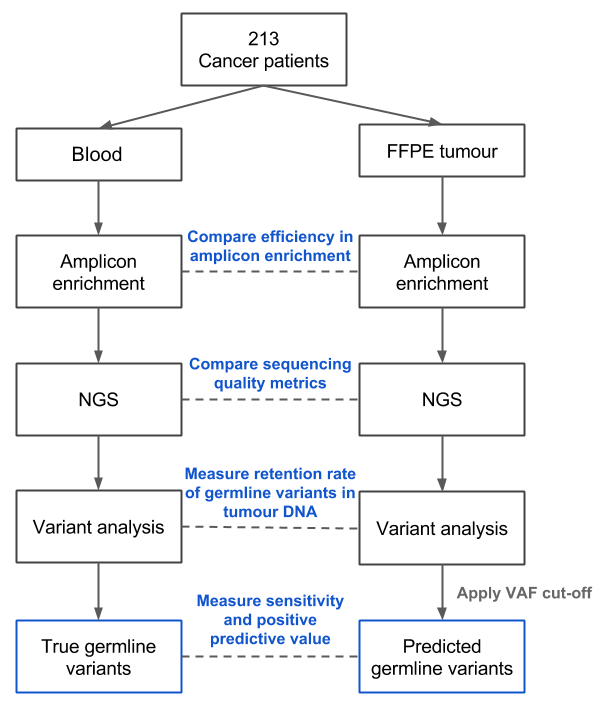
\includegraphics[scale=0.5]{study_design.png}
	\caption{Schematic description of study design and data analyses.}
	\label{fig:study_design}
\end{figure}

%%%%%%%%%%%%%%%%%%%%%%%%%%%%%%%%%%%%%%%%%%%%%%%%%%%%%%%%%%%%%%%%%%%%%
%%%%%%%%%%%%%%%%%%%%%%%%%%%%%%%%%%%%%%%%%%%%%%%%%%%%%%%%%%%%%%%%%%%%%

%%%%%%%%%%%%%%%%%%%%%%%%%%%%%%%%%%%%%%%%%%%%%%%%%%%%%%%%%%%%%%%%%%%%%%
\section{Patient samples}
\label{sec:Patientsamples}

Blood and FFPE tumour samples were acquired from 213 patients who provided informed consent for The OncoPanel Pilot (TOP) study (Human Research Ethics Protocol H14­-01212), a pilot study to optimize the OncoPanel, which is an amplicon-based targeted NGS panel for solid tumours. The TOP study also aims to assess the OncoPanel's application for guiding disease management and therapeutic intervention. One blood sample and four FFPE tumours were sequenced in duplicates, which resulted in 217 tumour-normal paired samples (434 sequencing libraries were included in our analyses). Patients in the TOP study are those with advanced cancers including CRC, lung cancer, melanoma, gastrointestinal stromal tumour (\acs{GIST}), and other cancers (\autoref{tbl:cancertypes}). The age of paraffin block for tumour samples ranges from 18 to 5356 days with a median of 274 days.

%%%%%%%%%%%%%%%%%%%%%%%%%%%%%%%%%%%%%%%%%%%%%%%%%%%%%%%%%%%%%%%%%%%%%%
%%%%%%%%%%%%%%%%%%%%%%%%%%%%%%%%%%%%%%%%%%%%%%%%%%%%%%%%%%%%%%%%%%%%%%
\begin{table}[H]
\caption{Distribution of cancer types in the TOP cohort.}
\label{tbl:cancertypes}
\centering
      \begin{tabular}{lccc}
        \hline
        Cancer Type & Number of Cases & Percentage (\%) \\ \hline
        Colorectal & 97 & 46 \\
        Lung & 60 & 28 \\
        Melanoma & 18 & 8 \\
				Other\textsuperscript{$\dagger$} & 16 & 8 \\
				GIST & 7 & 3 \\
				Sarcoma & 4 & 2 \\
				Neuroendocrine & 4 & 2 \\
				Cervical & 2 & 0.9 \\
				Ovarian & 2 & 0.9 \\
				Breast & 2 & 0.9 \\
				Unknown & 1 & 0.5 \\ \hline
      \end{tabular} \\
			\vspace{0.5cm}
\justify
{\small \textsuperscript{$\dagger$}This category includes thyroid, peritoneum, Fallopian tube, gastric, endometrial, squamous cell carcinoma, anal, salivary gland, peritoneal epithelial mesothelioma, adenoid cystic carcinoma, pancreas, breast, gall bladder, parotid epithelial myoepithelial carcinoma, carcinoid, and small bowel cancers.}
\end{table}

%%%%%%%%%%%%%%%%%%%%%%%%%%%%%%%%%%%%%%%%%%%%%%%%%%%%%%%%%%%%%%%%%%%%%%
\section{Sample preparation, library construction, and Illumina sequencing}
\label{sec:Samplepreparation,libraryconstruction,andIlluminasequencing}

Genomic DNA was extracted from blood and FFPE tumour samples using the Gentra Autopure LS DNA preparation platform and QIAamp DNA FFPE tissue kit (Qiagen, Hilden, Germany), respectively. The extracted DNA was sheared according to a previously described protocol \cite{Bosdet2013} to obtain approximate sizes of 3 kb followed by PCR primer merging, amplification of target regions, and adapter ligation using the Thunderstorm NGS Targeted Enrichment System (RainDance Technologies, Lexington, MA) as per manufacturer's protocol. Barcoded amplicons were sequenced with the Illumina MiSeq system for paired end sequencing with a v2 250-bp kit (Illumina, San Diego, CA).

%%%%%%%%%%%%%%%%%%%%%%%%%%%%%%%%%%%%%%%%%%%%%%%%%%%%%%%%%%%%%%%%%%%%%
\newpage
\section{OncoPanel (Amplicon-based targeted sequencing panel for solid tumours)}
\label{sec:OncoPanel}

The OncoPanel assesses coding exons and clinically relevant hotpots of 15 cancer-related genes and six PGx genes that can predict risk of developing chemotherapy-induced toxicity. Primers were designed by RainDance Technologies (Lexington, MA) using the GRCh37/hg19 human reference genome to generate 416 amplicons between 56 bp and 288 bp in size, which interrogate $\sim$20 kb of target bases. Complete list of genes and gene reference models for the OncoPanel is presented in \autoref{tbl:genemodel}, whereas OncoPanel target regions and amplicons are presented in \autoref{tbl:amplicons_target_regions}.

\normalsize
\begin{table}[H]
    \caption{Gene reference models for HGVS nomenclature of OncoPanel genes.}
    \label{tbl:genemodel}
    \centering
    \begin{tabular}{llll}
    \hline
    Gene & Protein & Reference Model \\
    \hline
    \multicolumn{3}{l}{\textit{Cancer-related}}
    \\
    AKT1 & Protein kinase B & NM\_001014431.1 \\
    ALK & Anaplastic lymphoma receptor tyrosine kinase & NM\_004304.3 \\
    BRAF & Serine/threonine-protein kinase B-Raf & NM\_004333.4 \\
    EGFR & Epidermal growth factor receptor & NM\_005228.3 \\
    HRAS & GTPase HRas & NM\_005343.2 \\
    MAPK1 & Mitogen-activated protein kinase 1 & NM\_002745.4 \\
    MAP2K1 & Mitogen-activated protein kinase kinase 1 & NM\_002755.3 \\
    MTOR & Serine/threonine-protein kinase mTOR & NM\_004958.3 \\
    NRAS & Neuroblastoma RAS viral oncogene homolog & NM\_002524.3 \\
    PDGFRA & Platelet-derived growth factor receptor alpha & NM\_006206.4 \\
    PIK3CA & Phosphatidylinositol-4,5-bisphosphate 3-kinase catalytic subunit alpha & NM\_006218.2 \\
    PTEN & Phosphatase and tensin homolog & NM\_000314.4 \\
    STAT1 & Signal transducer and activator of transcription 1 & NM\_007315.3 \\
    STAT3 & Signal transducer and activator of transcription 3 & NM\_139276.2 \\
    TP53 & Tumor protein P53 & NM\_000546.5 \\
    \\
    \multicolumn{3}{l}{\textit{Pharmacogenomics}}
    \\
    DPYD & Dihydropyrimidine dehydrogenase & NM\_000110.3 \\
    GSTP1 & Glutathione S-rransferase pi 1 & NM\_000852.3 \\
    MTHFR & Methylenetetrahydrofolate reductase & NM\_005957.4 \\
    TYMP & Thymidine phosphorylase & NM\_001113755.2 \\
    TYMS & Thymidylate synthetase & NM\_001071.2 \\
    UGT1A1 & Uridine diphosphate (UDP)-glucuronosyl transferase 1A1 & NM\_000463.2\\
    \hline
    \end{tabular}
\end{table}


%%%%%%%%%%%%%%%%%%%%%%%%%%%%%%%%%%%%%%%%%%%%%%%%%%%%%%%%%%%%%%%%%%%%%%
\section{Variant calling pipeline}
\label{sec:Variantcallingpipeline}

\subsection{Read alignment and variant calling}

Reads that passed the Illumina Chastity filter were aligned to the hg19 human reference genome using the \acs{BWA} mem algorithm (version 0.5.9) with default parameters, and the alignments were processed and converted to the BAM format using SAMtools (version 0.1.18). The SAMtools \texttt{mpileup} function \texttt{(samtools mpileup -BA -d 500000 -L 500000 -q 1)} was used to generate pileup files for all target bases followed by variant calling with the VarScan2 \texttt{mpileup2cns} (version 2.3.6) function with parameter thresholds of VAF $\geq$ 10\% and Phred-scaled BAQ score $\geq$ 20 \texttt{(--min-var-freq 0.1 --min-avg-qual 20 --strand-filter 0 --p-value 0.01 --output-vcf --variants)}.

Four genomic positions at which the hg19 human reference genome contains potential risk alleles were identified (\autoref{tbl:potential_risk_alleles}). Hence, patients homozygous for these four risk alleles would not be identified by our standard variant calling procedure. For these four genomic sites, our method for variant calling was modified to provide calls for every patient in the cohort. The VarScan2 \texttt{mpileup2cns} function with parameter thresholds of VAF $\geq$ 25\%, VAF to call homozygote $\geq$ 90\%, BAQ score $\geq$ 20, and fraction of variant reads from each strand $\geq$ 0.1 \texttt{(--min-var-freq 0.25 --min-freq-for-hom 0.9 --min-avg-qual 20 --strand-filter 1 \\--p-value 0.01 --output-vcf)} was used. Next, allelic statuses were re-assigned, in which wild type calls were re-assigned as homozygous variants, while homozygous variants were re-assigned as wild type calls. Corrections to the VAFs of these four genomic sites were also made to ensure that the VAFs reflect percentage of reads with the risk alleles.

%%%%%%%%%%%%%%%%%%%%%%%%%%%%%%%%%%%%%%%%%%%%%%%%%%%%%%%%%%%%%%%%%%%%%%
%%%%%%%%%%%%%%%%%%%%%%%%%%%%%%%%%%%%%%%%%%%%%%%%%%%%%%%%%%%%%%%%%%%%%%

\begin{longtable}{p{0.08\linewidth}|p{0.05\linewidth}p{0.1\linewidth}p{0.13\linewidth}p{0.16\linewidth}p{0.2\linewidth}}
    \caption{Potential risk alleles in the hg19 human reference genome within the target regions of the OncoPanel.}
    \label{tbl:potential_risk_alleles}
        \\
        \hline
        Gene & Chr & Pos & Risk Allele & dbSNP ID & HGVS\textsuperscript{*}
				\\
				\hline
        DPYD & chr1 & 98348885 & C & rs1801265 & p.Cys29Arg c.85T$>$C
        \\
        MTOR & chr1 & 11205058 & G & rs386514433; rs1057079 & p.Ala1577Ala c.4731A$>$G
        \\
        & chr1 & 11288758 & C & rs1064261 & p.Asn999Asn c.2997T$>$C
        \\
        TP53 & chr17 & 7579472 & C & rs1042522 & p.Arg72Pro c.215G$>$C
        \\
				\hline
\end{longtable}
\textsuperscript{*}Description of sequence variants according to the HGVS recommendations.

%%%%%%%%%%%%%%%%%%%%%%%%%%%%%%%%%%%%%%%%%%%%%%%%%%%%%%%%%%%%%%%%%%%%%%
%%%%%%%%%%%%%%%%%%%%%%%%%%%%%%%%%%%%%%%%%%%%%%%%%%%%%%%%%%%%%%%%%%%%%%

\subsection{Variant filtering}

Variant calls were filtered using the VarScan2 \texttt{fpfilter} function with fraction of variant reads from each strand $\geq$ 0.1 and default thresholds for other parameters (\autoref{tbl:varscan_fpfilter_parameters}). The VarScan2 \texttt{fpfilter} removed 247 low quality variants. Seventy germline variants in the blood were also excluded from our analysis because these variants in the tumours were filtered by the VarScan2 \texttt{fpfilter}. There were also 16 risk allele calls in tumour samples that did not pass the strand filter, causing the removal of 10 risk allele calls in the blood samples from our evaluation. Overall, a total of 343 calls were excluded by the VarScan2 \texttt{fpfilter} and strand filter. Manual inspection was performed for a subset of variants, including variants detected within primer regions and in PGx genes, using the Intergrative Genomics Viewer (IGV, version 2.3). This resulted in the removal of 500 spurious calls, which stemmed from software bugs, sequencing artifacts, primer masking, and primer artifacts (\autoref{tbl:spurious_calls}). Eleven low coverage calls ($\leq$ 100x) were also excluded from our analysis. Implementation of this filtering pipeline reduced the raw variant output of 5288 calls from 217 paired tumour-blood samples (434 sequencing libraries) to 4434 calls (\autoref{fig:variant_pipeline}B).

%%%%%%%%%%%%%%%%%%%%%%%%%%%%%%%%%%%%%%%%%%%%%%%%%%%%%%%%%%%%%%%%%%%%%%
%%%%%%%%%%%%%%%%%%%%%%%%%%%%%%%%%%%%%%%%%%%%%%%%%%%%%%%%%%%%%%%%%%%%%%

\begin{table}[H]
\caption{Thresholds for parameters of VarScan2 \texttt{fpfilter} used for filtering raw variant output.}
\label{tbl:varscan_fpfilter_parameters}
\centering
      \begin{tabular}{p{0.3\linewidth}p{0.56\linewidth}cp{0.1\linewidth}}
        \hline
        Parameter & Description & Threshold
				\\
				\hline
				\texttt{--min-var-count} & Min number of var-supporting reads & 4
				\\
        \texttt{--min-var-count-lc} & Min number of var-supporting reads when depth below somaticPdepth & 2
        \\
        \texttt{--min-var-freq} & Min variant allele frequency & 0.1
				\\
        \texttt{--max-somatic-p} & Max somatic p-value & 0.05
				\\
        \texttt{--max-somatic-p-depth} & Depth required to test max somatic p-value & 10
				\\
        \texttt{--min-ref-readpos} & Min average read position of ref-supporting reads & 0.1
				\\
        \texttt{--min-var-readpos} & Min average read position of var-supporting reads & 0.1
				\\
        \texttt{--min-ref-dist3} & Min average distance to effective 3' end of ref reads & 0.1
				\\
        \texttt{--min-var-dist3} & Min average distance to effective 3' end of variant reads & 0.1
				\\
        \texttt{--min-strandedness} & Min fraction of variant reads from each strand & 0.1
				\\
        \texttt{--min-strand-reads} & Min allele depth required to perform the strand tests & 5
				\\
        \texttt{--min-ref-basequal} & Min average base quality for ref allele & 15
				\\
        \texttt{--min-var-basequal} & Min average base quality for var allele & 15
				\\
        \texttt{--min-ref-avgrl} & Min average trimmed read length for ref allele & 90
				\\
        \texttt{--min-var-avgrl} & Min average trimmed read length for var allele & 90
        \\
        \texttt{--max-rl-diff} & Max average relative read length difference (ref - var) & 0.25
        \\
        \texttt{--max-ref-mmqs} & Max mismatch quality sum of ref-supporting reads & 100
        \\
        \texttt{--max-var-mmqs} & Max mismatch quality sum of var-supporting reads & 100
        \\
        \texttt{--max-mmqs-diff} & Max average mismatch quality sum (var - ref) & 50
        \\
        \texttt{--min-ref-mapqual} & Min average mapping quality for ref allele & 15
        \\
        \texttt{--min-var-mapqual} & Min average mapping quality for var allele & 15
        \\
        \texttt{--max-mapqual-diff} & Max average mapping quality (ref - var) & 50
        \\
				\hline
      \end{tabular}
\end{table}

%%%%%%%%%%%%%%%%%%%%%%%%%%%%%%%%%%%%%%%%%%%%%%%%%%%%%%%%%%%%%%%%%%%%%%
%%%%%%%%%%%%%%%%%%%%%%%%%%%%%%%%%%%%%%%%%%%%%%%%%%%%%%%%%%%%%%%%%%%%%%

\subsection{Variant annotation and interpretation}

SnpEff (version 4.2) was used for effect prediction, and the SnpSift package in SnpEff was used to annotate variants with databases such as dbSNP (b138), COSMIC (version 70), 1000 Genomes Project, and \acs{ExAC} (release 0.3) for interpretation. Clinical significance reported by the ClinVar database and literature review were also used for variant interpretation.

%%%%%%%%%%%%%%%%%%%%%%%%%%%%%%%%%%%%%%%%%%%%%%%%%%%%%%%%%%%%%%%%%%%%%%
%%%%%%%%%%%%%%%%%%%%%%%%%%%%%%%%%%%%%%%%%%%%%%%%%%%%%%%%%%%%%%%%%%%%%%

\newpage
\begin{longtable}{p{0.08\linewidth}p{0.05\linewidth}p{0.1\linewidth}p{0.04\linewidth}p{0.04\linewidth}p{0.6\linewidth}}
    \caption{Spurious variants removed by the variant filtering pipeline.}
    \label{tbl:spurious_calls}
        \\
        \hline
        Gene & Chr & Pos & Ref & Alt & Reason
				\\
				\hline
				KIT & chr4 & 55599268 & C & T & Variant masked by primer in FFPE specimen
				\\
        MAPK1 & chr22 & 22162126 & A & G & Variant masked by primer in FFPE specimen
        \\
        MTOR & chr1 & 11186783 & G & A & Sequencing artifact within primer region
        \\
        MTOR & chr1 & 11190646 & G & A & Variant masked by primer in FFPE specimen
        \\
        TYMP & chr22 & 50964446 & A & T & Poor target region, alignment of different sized amplicons
        \\
        TYMP & chr22 & 50964862 & A & T & Poor target region, alignment of different sized amplicons
        \\
        TYMS & chr18 & 673449 & G & C & VarScan2 bug after chr18:673443 c.*447\_*452delTTAAAG
        \\
        UGT1A1 & chr2 & 234668879 & CAT & C & Sequencing artifact at AT repeats in promoter
        \\
        UGT1A1 & chr2 & 234668881 & T & TAC & VarScan2 bug after AT insertion in promoter
        \\
				\hline
\end{longtable}

%%%%%%%%%%%%%%%%%%%%%%%%%%%%%%%%%%%%%%%%%%%%%%%%%%%%%%%%%%%%%%%%%%%%%%
%%%%%%%%%%%%%%%%%%%%%%%%%%%%%%%%%%%%%%%%%%%%%%%%%%%%%%%%%%%%%%%%%%%%%%

\begin{figure}[H]
\centering
	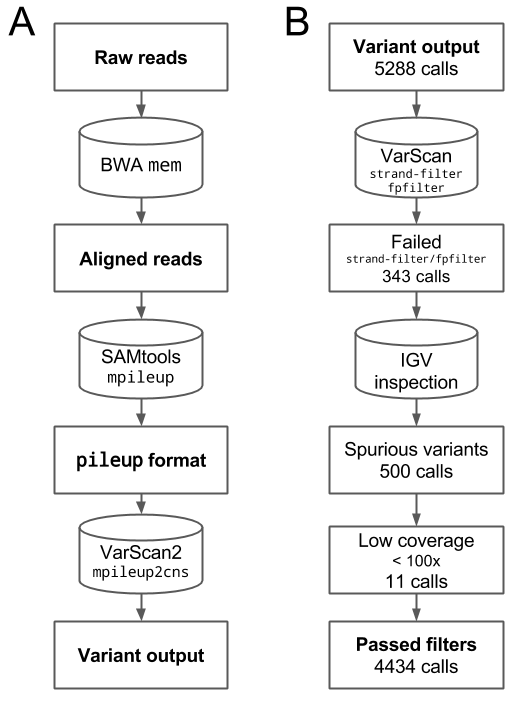
\includegraphics[scale=0.55]{variant_pipeline3.png}
	\caption{Pipelines for (A) variant calling and (B) filtering.}
	\label{fig:variant_pipeline}
\end{figure}

%%%%%%%%%%%%%%%%%%%%%%%%%%%%%%%%%%%%%%%%%%%%%%%%%%%%%%%%%%%%%%%%%%%%%%
\newpage
\section{Sequence analysis}
\label{sec:Sequenceanalysis}

A custom Python script was used to process BAM files to quantify the number of on-target aligned (reads that map to target regions), off-target aligned (reads that map to hg19 but not target regions), and unaligned reads with a Phred-scaled mapping quality (\acs{MAPQ}) score $\geq$ 10. Unaligned reads were also screened against microbial sequences, including viruses, archaea, bacteria, and fungi, to ensure that samples do not contain significant amount of microbial contaminants. Coverage depth for target bases with MAPQ $\geq$ 1 and BAQ $\geq$ 20 was obtained using bam-readcount (https://github.com/genome/bam-readcount). To measure coverage depth of amplicons, the SAMtools \texttt{view} function was used to filter for reads with MAPQ $\geq$ 1 \texttt{(samtools view -b -q 1)} followed by the bedtools \texttt{intersect} function (version 2.25.0) to quantify the number of reads that overlap with amplicon positions \texttt{(intersect -a \$AMPLICON\_POSITIONS -b \$BAM\_FILE -f 0.95 -r -c)}.

Per-base metrics generated using bam-readcount were also used for assessment of sequence artifacts. A custom R script was used to count and categorize the different groups of base changes (i.e. C$>$T/G$>$A, A$>$G/T$>$C, C$>$A/G$>$T, A$>$C/T$>$G, C$>$G/G$>$C, and A$>$T/T$>$A). Unless stated otherwise, analysis of sequence artifacts excludes true variants identified by our VarScan2 variant calling pipeline and base changes with VAF $<$ 1\%, which are considered sequencing errors. All statistical analyses and data visualization were performed using the R statistical software package (version 3.3.2) and associated open-source packages.

%%%%%%%%%%%%%%%%%%%%%%%%%%%%%%%%%%%%%%%%%%%%%%%%%%%%%%%%%%%%%%%%%%%%%%
\section{Application of VAF thresholds to separate germline alterations from somatic mutations}
\label{sec:ApplicationofVAFthresholdstoseparategermlinealterationsfromsomaticmutations}

Variants in the tumours that passed our filtering criteria were subjected to VAF thresholds between 10--45\%. At each VAF cut-off, variants that were not filtered out were considered predicted germline variants. Given that all tumour samples have matched blood samples, true positives were identified as predicted germline variants that overlap with variants in the blood (\autoref{fig:tpfptnfn}). Conversely, false negatives were identified as variants that were filtered out by the VAF cut-off (predicted as somatic), but were present in the blood samples. Sensitivity at each VAF threshold was calculated by dividing the number of true positives with the sum of true positives and false negatives. Because predicted germline variants will be referred to follow-up germline testing, positive predictive values (\acs{PPV}s) were calculated at each VAF cut-off to evaluate precision of our approach. False positives were identified as predicted germline variants that were absent in the blood, and PPV was calculated by dividing the number of true positives with the sum of true positives and false positives.

%%%%%%%%%%%%%%%%%%%%%%%%%%%%%%%%%%%%%%%%%%%%%%%%%%%%%%%%%%%%%%%%%%%%%%
%%%%%%%%%%%%%%%%%%%%%%%%%%%%%%%%%%%%%%%%%%%%%%%%%%%%%%%%%%%%%%%%%%%%%%

\begin{figure}[H]
\centering
	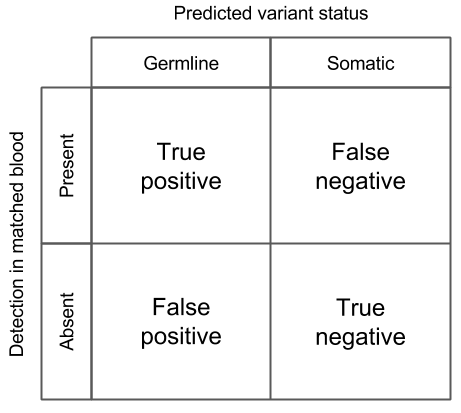
\includegraphics[scale=0.55]{tpfptnfn.png}
	\caption{2x2 contingency table for determination of true positive, false positive, true negative, and false negative variant calls in tumour-only analyses.}
	\label{fig:tpfptnfn}
\end{figure}


%%%%%%%%%%%%%%%%%%%%%%%%%%%%%%%%%%%%%%%%%%%%%%%%%%%%%%%%%%%%%%%%%%%%%%

\endinput
